\documentclass[11pt]{article}
\usepackage{amsmath, amssymb, physics, mathtools, bm}
\usepackage{tikz, pgfplots}
\pgfplotsset{compat=1.18}
\usepackage[margin=2.3cm]{geometry}
\usepackage{siunitx, booktabs, hyperref}
\usepackage{braket}

\newcommand{\D}{\mathrm{D}}
\newcommand{\de}{\mathrm{d}}
\newcommand{\pd}[2]{\frac{\partial #1}{\partial #2}}
\newcommand{\pdd}[2]{\frac{\partial^{2} #1}{\partial #2^{2}}}

\title{B5 General Relativity \& Cosmology --- Model Solutions, 2016}
\author{}
\date{}

\begin{document}
\maketitle

%==============================================================
\section*{Question 1 --- Schwarzschild orbits and circular geodesics}

\textbf{Problem.} Schwarzschild metric. Reduce to equatorial plane; find $\dot t$, $\dot\phi$ and the orbit equation $u'' + u = A + B u^2$. A satellite is launched azimuthally from a stationary station at $r=R$ with locally measured speed $v_\text{circ}$ giving a circular orbit. Find $v_\text{circ}$ and the time before the orbiting satellite collides with the station. Sketch the perturbed orbit when the launch speed is $v_\text{circ}+\Delta v$.

\subsection*{(a) Equatorial reduction and conserved quantities}

The metric is spherically symmetric, so it is invariant under $\theta\to\pi-\theta$. Pick initial conditions with $\theta=\pi/2$, $\dot\theta=0$ (always possible by rotation): the Euler--Lagrange equation for $\theta$ has the right-hand side proportional to $\sin\theta\cos\theta\,\dot\phi^2$, vanishing on the equator. Hence $\theta(\tau)\equiv\pi/2$ is a geodesic; restricting to it loses no generality.

Lagrangian per unit rest mass on the equator (using $\dot{\,}=\de/\de\tau$):
\begin{equation}
\mathcal L = -\!\left(1-\tfrac{2GM}{c^2 r}\right)\!c^2\dot t^{\,2} + \!\left(1-\tfrac{2GM}{c^2 r}\right)^{\!-1}\!\dot r^{\,2} + r^2\dot\phi^{\,2}.
\label{eq:lag}
\end{equation}
$\mathcal L$ has no explicit $t$ or $\phi$:
\[
\pd{\mathcal L}{\dot t} = -2c^2\!\left(1-\tfrac{2GM}{c^2 r}\right)\!\dot t = \text{const},
\]
\[
\pd{\mathcal L}{\dot\phi} = 2 r^2\dot\phi = \text{const}.
\]
Define the two constants of motion (energy $E$ and angular momentum $\ell$ per unit rest mass):
\begin{equation}
\boxed{\;\!\left(1-\tfrac{2GM}{c^2 r}\right)\!\dot t = \frac{E}{c^2},\qquad r^2\dot\phi = \ell.\;}
\label{eq:Eell}
\end{equation}

\subsection*{(b) Radial equation and orbit equation}

Normalisation of the 4-velocity, $g_{ab}\dot x^a\dot x^b = -c^2$, on the equator:
\[
-\!\left(1-\tfrac{2GM}{c^2 r}\right)\!c^2\dot t^{\,2} + \!\left(1-\tfrac{2GM}{c^2 r}\right)^{\!-1}\!\dot r^{\,2} + r^2\dot\phi^{\,2} = -c^2.
\]
Substitute \eqref{eq:Eell}:
\[
-\frac{E^2/c^2}{1-2GM/(c^2 r)} + \frac{\dot r^{\,2}}{1-2GM/(c^2 r)} + \frac{\ell^2}{r^2} = -c^2.
\]
Multiply by $1-2GM/(c^2 r)$ and rearrange:
\begin{equation}
\boxed{\;\dot r^{\,2} = \frac{E^2}{c^2} - \!\left(1-\tfrac{2GM}{c^2 r}\right)\!\!\left(c^2 + \frac{\ell^2}{r^2}\right).\;}
\label{eq:rdot}
\end{equation}

Change variable to $u(\phi) = 1/r$. Use $\dot r = (\de r/\de\phi)\dot\phi = -u^{-2}u'\,\ell u^2 = -\ell u'$:
\[
\dot r^{\,2} = \ell^2 (u')^2.
\]
Insert into \eqref{eq:rdot}:
\[
\ell^2 (u')^2 = \frac{E^2}{c^2} - c^2 + \tfrac{2GM}{c^2}c^2 u - \ell^2 u^2 + \tfrac{2GM}{c^2}\ell^2 u^3.
\]
Differentiate w.r.t.\ $\phi$ and divide by $2 u'$:
\[
\ell^2 u'' = GM - \ell^2 u + 3 GM u^2.
\]
Divide by $\ell^2$:
\begin{equation}
\boxed{\;u'' + u = A + B u^2,\qquad A = \frac{GM}{\ell^2},\quad B = \frac{3GM}{c^2}.\;}
\label{eq:orbit}
\end{equation}

\subsection*{(c) Circular orbit launched from the station}

Circular orbit: $u = u_0 = 1/R$ constant, so \eqref{eq:orbit} gives $u_0 = A + B u_0^2$:
\[
\frac{1}{R} = \frac{GM}{\ell^2} + \frac{3GM}{c^2 R^2}.
\]
Solve for $\ell^2$:
\[
\ell^2 = \frac{GM\,R^2}{R - 3GM/c^2} = \frac{GMR^2}{R(1-3GM/(c^2 R))}.
\]
Cleaner form:
\begin{equation}
\ell^2 = \frac{GMR}{1 - 3GM/(c^2 R)}.
\label{eq:ell-circ}
\end{equation}

The astronaut's locally measured speed is the proper distance moved per unit proper time. The station is static at $r=R$, so the astronaut's frame uses
\[
\de\ell_\perp = R\,\de\phi,\qquad \de\tau_\text{stn} = \sqrt{1-\tfrac{2GM}{c^2 R}}\,\de t.
\]
The satellite passes the station with $\dot r=0$, $\dot\theta=0$, $\dot\phi\ne 0$. Local speed:
\[
v_\text{circ} = \frac{R\,\de\phi}{\de\tau_\text{stn}} = \frac{R\,\dot\phi}{\sqrt{1-2GM/(c^2 R)}\,\dot t}.
\]
From \eqref{eq:Eell}, $\dot\phi/\dot t = \ell c^2/(R^2 E)\cdot(1-2GM/(c^2 R))$. Use the alternative route: write $v_\text{circ}^2 = (R\,\de\phi/\de\tau_\text{stn})^2$. We have
\[
\frac{(R\,\de\phi)^2}{\de\tau_\text{stn}^2} = \frac{R^2 \dot\phi^2}{(1-2GM/(c^2 R))\,\dot t^{\,2}}.
\]
Multiply top and bottom by $\de\tau^2$ and use $r^2\dot\phi = \ell$:
\[
v_\text{circ}^2 = \frac{\ell^2/R^2}{(1-2GM/(c^2 R))\,\dot t^{\,2}/\de\tau^2}\cdot\frac{1}{R^2/R^2}.
\]
Cleaner: along the circular orbit, the 4-velocity normalisation reads
\[
-c^2 = -\!\left(1-\tfrac{2GM}{c^2 R}\right)\!c^2\dot t^{\,2} + R^2\dot\phi^{\,2}.
\]
Solve for $R^2\dot\phi^{\,2}$:
\[
R^2\dot\phi^{\,2} = \!\left(1-\tfrac{2GM}{c^2 R}\right)\!c^2\dot t^{\,2} - c^2.
\]
Divide by $(1-2GM/(c^2 R))\,\dot t^{\,2}$:
\[
v_\text{circ}^2 = \frac{R^2\dot\phi^{\,2}}{(1-2GM/(c^2 R))\,\dot t^{\,2}} = c^2 - \frac{c^2}{(1-2GM/(c^2 R))\,\dot t^{\,2}}.
\]
Use \eqref{eq:Eell}: $(1-2GM/(c^2 R))\,\dot t = E/c^2$, so $(1-2GM/(c^2 R))\,\dot t^{\,2} = E^2/[c^4(1-2GM/(c^2 R))]$. Cleaner: rewrite using $\ell = R^2\dot\phi$:
\[
v_\text{circ}^2 = \frac{\ell^2/R^2}{(1-2GM/(c^2 R))\,\dot t^{\,2}}.
\]
Expand $\dot t^{\,2}$ from the same normalisation: $\dot t^{\,2} = (1+\ell^2/(c^2 R^2))/(1-2GM/(c^2 R))$. Insert:
\[
v_\text{circ}^2 = \frac{\ell^2/R^2}{(1-2GM/(c^2 R))\cdot(1+\ell^2/(c^2 R^2))/(1-2GM/(c^2 R))} = \frac{\ell^2/R^2}{1 + \ell^2/(c^2 R^2)}.
\]
Substitute \eqref{eq:ell-circ}:
\[
\frac{\ell^2}{R^2} = \frac{GM/R}{1 - 3GM/(c^2 R)}.
\]
Numerator divided by $1+\ell^2/(c^2 R^2)$. Compute $\ell^2/(c^2 R^2) = (GM/(c^2 R))/(1-3GM/(c^2 R))$. Hence
\[
1 + \frac{\ell^2}{c^2 R^2} = \frac{1 - 3GM/(c^2 R) + GM/(c^2 R)}{1-3GM/(c^2 R)} = \frac{1 - 2GM/(c^2 R)}{1 - 3GM/(c^2 R)}.
\]
Divide:
\[
v_\text{circ}^2 = \frac{GM/R}{1-3GM/(c^2 R)}\cdot\frac{1-3GM/(c^2 R)}{1-2GM/(c^2 R)}.
\]
Simplify:
\begin{equation}
\boxed{\;v_\text{circ}^2 = \frac{GM/R}{1 - 2GM/(c^2 R)}.\;}
\label{eq:vcirc}
\end{equation}
Note the Newtonian limit $v_\text{circ}^2\to GM/R$ when $2GM/(c^2 R)\ll 1$.

\paragraph{Time to collision (in the astronaut's proper time).}
Orbital period in coordinate time: $T_t = 2\pi/\dot\phi\cdot(\dot t/1)$, but easier to relate proper times directly. Proper-time period of the satellite over one revolution:
\[
T_\text{sat} = 2\pi/\dot\phi = 2\pi R^2/\ell.
\]
Substitute \eqref{eq:ell-circ}:
\[
T_\text{sat} = 2\pi R^2/\sqrt{GMR/(1-3GM/(c^2 R))} = 2\pi\sqrt{R^3/GM}\,\sqrt{1-3GM/(c^2 R)}.
\]
Convert to station proper time via $\de\tau_\text{stn} = \sqrt{1-2GM/(c^2 R)}\,\de t$ and $\de t/\de\tau_\text{sat} = \dot t$. Use \eqref{eq:Eell}:
\[
\dot t = \frac{E/c^2}{1-2GM/(c^2 R)}.
\]
Energy from $\dot t^{\,2} = (1+\ell^2/(c^2 R^2))/(1-2GM/(c^2 R))$ and $E = c^2(1-2GM/(c^2 R))\dot t$:
\[
E^2/c^4 = (1-2GM/(c^2 R))(1+\ell^2/(c^2 R^2)) = \frac{(1-2GM/(c^2 R))^2}{1-3GM/(c^2 R)}.
\]
Coordinate-time period: $T_t = T_\text{sat}\,\dot t = T_\text{sat}\cdot E/[c^2(1-2GM/(c^2 R))]$. Combine:
\[
T_t = 2\pi\sqrt{R^3/GM}\,\sqrt{1-3GM/(c^2 R)}\cdot\frac{E/c^2}{1-2GM/(c^2 R)}.
\]
Insert $E/c^2 = (1-2GM/(c^2 R))/\sqrt{1-3GM/(c^2 R)}$:
\[
T_t = 2\pi\sqrt{R^3/GM}.
\]
This is exactly Kepler's third law in coordinate time. Now convert to station proper time:
\[
T_\text{stn} = T_t\sqrt{1-2GM/(c^2 R)}.
\]
\begin{equation}
\boxed{\;T_\text{stn} = 2\pi\sqrt{\frac{R^3}{GM}}\,\sqrt{1-\frac{2GM}{c^2 R}}.\;}
\label{eq:Tstn}
\end{equation}
Newtonian limit: $T_\text{stn}\to 2\pi\sqrt{R^3/GM}$. Strong-field correction: time runs slower at the station than at infinity, so the wait is shorter than Kepler's value.

\subsection*{(d) Perturbed launch}

For $|\Delta v|\ll v_\text{circ}$ the orbit is a near-circular ellipse: writing $u = u_0 + \delta u$ in \eqref{eq:orbit} and linearising,
\[
\delta u'' + (1 - 2 B u_0)\,\delta u = 0.
\]
Substitute $B u_0 = 3GM/(c^2 R)$:
\[
\delta u'' + \!\left(1-\tfrac{6GM}{c^2 R}\right)\!\delta u = 0.
\]
Apsidal precession frequency (per orbit) is $\sqrt{1-6GM/(c^2 R)} < 1$, so radial oscillations close in azimuthal angle $2\pi/\sqrt{1-6GM/(c^2 R)} > 2\pi$: each radial period the perihelion advances by
\[
\Delta\phi_\text{prec} \approx \pi\,\frac{6GM}{c^2 R}.
\]

\begin{center}
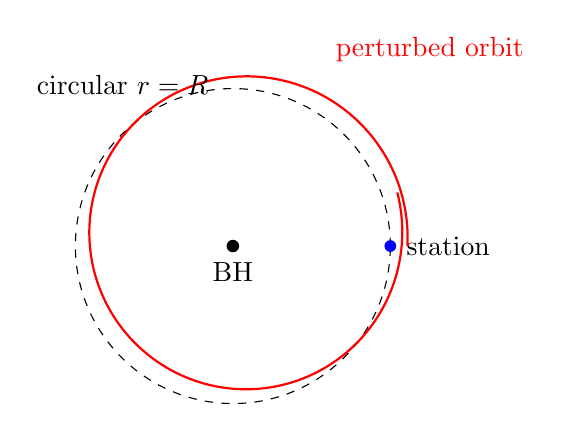
\begin{tikzpicture}[>=stealth, scale=1.0]
  \node[circle,fill=black,inner sep=1.6pt,label=below:{BH}] (BH) at (0,0) {};
  \draw[dashed] (0,0) circle (2.0cm);
  \node[circle,fill=blue,inner sep=1.5pt,label=right:{station}] (S) at (2.0,0) {};
  \draw[thick,red,domain=0:6.6,samples=200,smooth] plot ({(2.0+0.25*cos(\x*180/3.14*0.93 - 30))*cos(\x r)},
                                                          {(2.0+0.25*cos(\x*180/3.14*0.93 - 30))*sin(\x r)});
  \node[red] at (2.5,2.5) {perturbed orbit};
  \node[above] at (-1.4,1.8) {circular $r=R$};
\end{tikzpicture}
\end{center}

The orbit oscillates between $r_-<R<r_+$, with the line of apsides precessing forward; for $\Delta v\ne 0$ the satellite returns to $r=R$ but at a shifted azimuth, so it does \emph{not} hit the station on the first pass. However the perihelion drifts secularly, and after $\sim 2\pi/\Delta\phi_\text{prec}$ radial periods the apse returns to the station's azimuth: the station is therefore \emph{not} safe forever --- collision occurs after a finite (but long) time. (Strictly true outside the ISCO at $r = 6GM/c^2$; below this the perturbation is unstable and collision is rapid.)

%==============================================================
\section*{Question 2 --- Einstein equations and TOV; uniform-density star}

\textbf{Problem.} Argue $G_{ab} = R_{ab}-\tfrac12 g_{ab}R$. For a static spherical metric reduce $G_{ab}=-(8\pi G/c^4)T_{ab}$ to the TOV equations. For a uniform-density star derive $p_0(R)$ and the Buchdahl bound $2GM/(c^2 R) < 8/9$. Comment on a redshift $z=3.1$ neutron star.

\subsection*{(a) Form of the Einstein tensor}

Energy--momentum conservation in curved space requires $\nabla_a T^{ab} = 0$. If $G^{ab}\propto T^{ab}$ then $\nabla_a G^{ab} = 0$.

The Ricci tensor alone fails: the contracted Bianchi identity gives $\nabla_a R^{ab} = \tfrac12\nabla^b R\ne 0$. Subtract the trace to enforce conservation:
\[
G_{ab} = R_{ab} - \tfrac12 g_{ab} R.
\]
Bianchi identity then yields $\nabla^a G_{ab} \equiv 0$. $G_{ab}$ is symmetric (both $R_{ab}$ and $g_{ab}$ are) and built from the metric and its first two derivatives, matching the second-derivative structure of $T_{ab}$ (Newtonian limit: Poisson). The proportionality constant is fixed by Newtonian limit to $-8\pi G/c^4$:
\[
\boxed{\;G_{ab} = R_{ab}-\tfrac12 g_{ab}R = -\tfrac{8\pi G}{c^4}T_{ab}.\;}
\]

\subsection*{(b) Static fluid: 4-velocity components}

In the given coordinates $G_{ab}$ is diagonal; for a perfect fluid \eqref{eq:Tdef-implicit} below
\[
T^{ab} = (\rho + p/c^2) u^a u^b + g^{ab} p, \tag{1}\label{eq:Tdef-implicit}
\]
gives off-diagonal $T^{0i}\propto u^0 u^i$. Diagonality of $G_{ab}$ forces $u^1=u^2=u^3=0$. The fluid is comoving with the static frame.

Normalisation $u^a u_a = -c^2$:
\[
g_{00}(u^0)^2 = -c^2 \;\Rightarrow\; -e^{2\Phi}(u^0)^2 = -c^2.
\]
Solve:
\[
\boxed{\;u^0 = c\,e^{-\Phi},\qquad u_0 = g_{00}u^0 = -c\,e^{\Phi}.\;}
\]

\subsection*{(c) The 00 equation: enclosed-mass form of $\Lambda(r)$}

$T_{00} = (\rho+p/c^2) u_0 u_0 + g_{00}p = (\rho c^2)\,e^{2\Phi}$. (Cross term: $(\rho+p/c^2)c^2 e^{2\Phi} - p e^{2\Phi} = \rho c^2 e^{2\Phi}$.)
Field equation:
\[
G_{00} = -\tfrac{8\pi G}{c^4}\rho c^2 e^{2\Phi}.
\]
Substitute the given $G_{00}$:
\[
-\frac{e^{2\Phi}}{r^2}\,\frac{\de}{\de r}\!\left[r(1-e^{-2\Lambda})\right] = -\tfrac{8\pi G}{c^2}\rho\, e^{2\Phi}.
\]
Cancel $e^{2\Phi}$ and rearrange:
\[
\frac{\de}{\de r}\!\left[r(1-e^{-2\Lambda})\right] = \tfrac{8\pi G}{c^2}\rho\,r^2.
\]
Integrate from $0$ to $r$ with $r(1-e^{-2\Lambda})\to 0$ at the origin:
\[
r(1-e^{-2\Lambda}) = \tfrac{8\pi G}{c^2}\!\int_0^r \rho(r')r'^2\,\de r' = \frac{2GM(r)}{c^2}.
\]
Solve for $e^{-2\Lambda}$:
\begin{equation}
\boxed{\;e^{-2\Lambda(r)} = 1 - \frac{2GM(r)}{c^2 r}.\;}
\label{eq:Lambda}
\end{equation}

\subsection*{(d) The 11 equation: $\de\Phi/\de r$}

$T_{11} = g_{11}p = e^{2\Lambda}p$. Field equation:
\[
G_{11} = -\tfrac{8\pi G}{c^4}e^{2\Lambda}p.
\]
Substitute given $G_{11}$:
\[
\frac{e^{2\Lambda}}{r^2} - \frac{1}{r^2} - \frac{2\Phi'}{r} = -\tfrac{8\pi G}{c^4}e^{2\Lambda}p.
\]
Multiply by $r^2 e^{-2\Lambda}$:
\[
1 - e^{-2\Lambda} - 2 r\,\Phi' e^{-2\Lambda} = -\tfrac{8\pi G}{c^4}r^2 p \cdot \text{(wait: re-multiply carefully)}.
\]
Restart: rearrange the original equation algebraically. Multiply by $r$:
\[
\frac{e^{2\Lambda}}{r} - \frac{1}{r} - 2\Phi' = -\tfrac{8\pi G}{c^4}r\,e^{2\Lambda}p.
\]
Now multiply by $e^{-2\Lambda}$:
\[
\frac{1}{r} - \frac{e^{-2\Lambda}}{r} - 2\Phi' e^{-2\Lambda} = -\tfrac{8\pi G}{c^4}r\,p.
\]
Use \eqref{eq:Lambda}: $1-e^{-2\Lambda} = 2GM/(c^2 r)$. Hence $1/r - e^{-2\Lambda}/r = 2GM/(c^2 r^2)$:
\[
\frac{2GM(r)}{c^2 r^2} - 2\Phi' e^{-2\Lambda} = -\tfrac{8\pi G}{c^4}r\,p.
\]
Solve for $\Phi'$:
\[
2\Phi' e^{-2\Lambda} = \frac{2GM(r)}{c^2 r^2} + \frac{8\pi G p\,r}{c^4}.
\]
Divide by $2 e^{-2\Lambda} = 2(1-2GM/(c^2 r))$:
\begin{equation}
\boxed{\;\frac{\de\Phi}{\de r} = \frac{GM(r) + 4\pi G p\,r^3/c^2}{c^2 r^2\bigl(1 - 2GM(r)/(c^2 r)\bigr)}.\;}
\label{eq:Phip}
\end{equation}

\subsection*{(e) TOV pressure equation}

Energy--momentum conservation (given):
\[
(\rho c^2 + p)\,\frac{\de\Phi}{\de r} = -\frac{\de p}{\de r}.
\]
Substitute \eqref{eq:Phip}:
\begin{equation}
\boxed{\;\frac{\de p}{\de r} = -(\rho c^2 + p)\,\frac{GM(r) + 4\pi G p\,r^3/c^2}{c^2 r^2\bigl(1 - 2GM(r)/(c^2 r)\bigr)}.\;}
\label{eq:TOV}
\end{equation}

\subsection*{(f) Uniform-density star: central pressure}

$\rho =$ const, so $M(r) = \tfrac{4}{3}\pi\rho r^3$ for $r\le R$.

Convenient combination: $4\pi G\rho/c^2 = 3 GM(R)/(c^2 R^3)\cdot 1$ (consistent). Define
\[
A \equiv \rho c^2,\qquad u(r) \equiv 2GM(r)/(c^2 r) = \frac{8\pi G\rho r^2}{3 c^2}.
\]
Plug into \eqref{eq:TOV}: numerator inside the bracket is $GM(r) + 4\pi G p\,r^3/c^2 = G\cdot\tfrac43\pi\rho r^3 + 4\pi G p r^3/c^2 = \tfrac{4\pi G r^3}{3 c^2}(\rho c^2 + 3p)$.
\[
\frac{\de p}{\de r} = -(\rho c^2 + p)\cdot\frac{4\pi G r^3(\rho c^2 + 3p)/(3 c^2)}{c^2 r^2(1 - u)} = -\frac{4\pi G r}{3 c^4}\cdot\frac{(\rho c^2+p)(\rho c^2 + 3p)}{1-u}.
\]
Use $1-u = 1 - 8\pi G\rho r^2/(3 c^2)$. Separate variables:
\[
\frac{\de p}{(\rho c^2 + p)(\rho c^2 + 3p)} = -\frac{4\pi G r/(3 c^4)}{1 - 8\pi G\rho r^2/(3 c^2)}\,\de r.
\]
RHS is exact: let $w = 1 - 8\pi G\rho r^2/(3 c^2)$, $\de w = -16\pi G\rho r/(3 c^2)\,\de r$:
\[
\text{RHS} = -\frac{4\pi G r}{3 c^4}\cdot\frac{1}{w}\,\de r = \frac{1}{4\rho c^2}\cdot\frac{\de w}{w}.
\]
Apply hint with $A = \rho c^2$, $x = p$:
\[
\int\frac{\de p}{(A+3p)(A+p)} = \frac{3}{2A}\!\int\frac{\de p}{A+3p} - \frac{1}{2A}\!\int\frac{\de p}{A+p} = \frac{1}{2A}\!\left[\ln(A+3p) - \ln(A+p)\right].
\]
Equate with LHS integrated:
\[
\frac{1}{2 A}\ln\!\frac{A+3p}{A+p} = \frac{1}{4 A}\ln w + \text{const}.
\]
Multiply by $2 A$:
\[
\ln\!\frac{A+3p}{A+p} = \tfrac12\ln w + \text{const}.
\]
Exponentiate:
\[
\frac{A+3p}{A+p} = K\sqrt{w}.
\]
Boundary at the surface $r=R$: $p(R) = 0$, $w(R) = 1 - 2GM/(c^2 R)$. Hence $K = 1/\sqrt{1-2GM/(c^2 R)}$. Total mass $M = \tfrac43\pi\rho R^3$.

At the centre $r = 0$: $w(0) = 1$, so
\[
\frac{A+3 p_0}{A + p_0} = \frac{1}{\sqrt{1-2GM/(c^2 R)}}.
\]
Solve for $p_0$. Cross-multiply:
\[
(A + 3 p_0)\sqrt{1-2GM/(c^2 R)} = A + p_0.
\]
Let $\sigma\equiv\sqrt{1-2GM/(c^2 R)}$:
\[
A\sigma + 3 p_0 \sigma = A + p_0.
\]
Group $p_0$ on one side:
\[
p_0(3\sigma - 1) = A(1 - \sigma).
\]
Solve and substitute $A = \rho c^2$:
\begin{equation}
\boxed{\;p_0 = \rho c^2\,\frac{1 - \sqrt{1 - 2GM/(c^2 R)}}{3\sqrt{1 - 2GM/(c^2 R)} - 1}.\;}
\label{eq:p0}
\end{equation}

\subsection*{(g) Buchdahl bound}

$p_0 \to \infty$ when the denominator of \eqref{eq:p0} vanishes:
\[
3\sqrt{1-2GM/(c^2 R)} = 1.
\]
Square:
\[
9(1-2GM/(c^2 R)) = 1.
\]
Solve:
\[
\frac{2GM}{c^2 R} = \frac{8}{9}.
\]
Hence the upper bound on the mass at fixed $R$:
\begin{equation}
\boxed{\;M < \frac{4 c^2 R}{9 G}.\;}
\label{eq:Buch}
\end{equation}

\subsection*{(h) Plausibility of $z = 3.1$}

Surface gravitational redshift in the Schwarzschild exterior:
\[
1 + z = \frac{1}{\sqrt{1 - 2GM/(c^2 R)}}.
\]
Solve for the compactness:
\[
\frac{2GM}{c^2 R} = 1 - \frac{1}{(1+z)^2}.
\]
At $z = 3.1$, $(1+z)^2 = 4.10^2 = 16.81$, so $1/(1+z)^2 = 0.0595$:
\[
\frac{2GM}{c^2 R} = 0.940.
\]
Compare with Buchdahl \eqref{eq:Buch}: $8/9 = 0.889$. Since $0.940 > 0.889$, the claimed redshift exceeds the maximum allowed by any static fluid configuration with $\rho\ge 0$ and $\rho$ non-increasing outwards.
\[
\boxed{\;\text{Claim implausible: } 2GM/(c^2 R) = 0.94 > 8/9.\;}
\]

%==============================================================
\section*{Question 3 --- FRW geometry and surface-brightness dimming}

\textbf{Problem.} Realise the 3-sphere line element; state flat and hyperbolic counterparts; quote $4\pi r^2$-style surface areas. Justify the FRW form. Derive cosmological redshift. Compute angular diameter $\Delta\theta$ and the surface-brightness scaling, and discuss telescope diameter for high-$z$ galaxies.

\subsection*{(a) The 3-sphere line element}

Parametrise $w^2+x^2+y^2+z^2 = A^2$ via
\[
w = A\cos\chi,\quad x = A\sin\chi\sin\theta\cos\phi,\quad y = A\sin\chi\sin\theta\sin\phi,\quad z = A\sin\chi\cos\theta,
\]
$\chi\in[0,\pi]$.
\[
\de w^2 + \de x^2 + \de y^2 + \de z^2 = A^2\bigl[\de\chi^2 + \sin^2\chi\,(\de\theta^2 + \sin^2\theta\,\de\phi^2)\bigr].
\]
Change to $\bar r \equiv A\sin\chi$:
\[
\de\bar r = A\cos\chi\,\de\chi,\qquad A^2\de\chi^2 = \frac{\de\bar r^2}{\cos^2\chi} = \frac{A^2\de\bar r^2}{A^2-\bar r^2}.
\]
Hence
\[
\boxed{\;\de s^2_{(+1)} = \frac{A^2}{A^2-\bar r^2}\,\de\bar r^2 + \bar r^2(\de\theta^2 + \sin^2\theta\,\de\phi^2).\;}
\]
Flat ($k=0$):
\[
\de s^2_{(0)} = \de\bar r^2 + \bar r^2(\de\theta^2 + \sin^2\theta\,\de\phi^2).
\]
Hyperbolic ($k=-1$): replace $\sin\chi\to\sinh\chi$; equivalently
\[
\de s^2_{(-1)} = \frac{A^2}{A^2+\bar r^2}\,\de\bar r^2 + \bar r^2(\de\theta^2 + \sin^2\theta\,\de\phi^2).
\]

\paragraph{Surface area of $\bar r=\bar R$.}
The induced $(\theta,\phi)$ metric is $\bar R^2(\de\theta^2+\sin^2\theta\,\de\phi^2)$ in all three cases:
\[
\boxed{\;\text{Area} = 4\pi \bar R^2 \quad \text{(flat, closed, open)}.\;}
\]
Geometry differs in the radial part, not in the area element.

\subsection*{(b) FRW from homogeneity and isotropy}

Cosmological principle: the spatial 3-geometry is maximally symmetric (isotropic at every point). The only such 3-geometries are flat $(k=0)$, 3-sphere $(k=+1)$ and 3-hyperboloid $(k=-1)$. Allow the overall length scale to depend on time, $a(t)$: the spatial part of the line element is $a^2(t)\,\de\sigma_k^2$. Combining all three $k$ cases by absorbing $A$ into $a$ and choosing $r$ such that the angular part is $a^2 r^2$:
\[
\de s^2 = -c^2\de t^2 + a^2(t)\!\left[\frac{\de r^2}{1-k r^2} + r^2(\de\theta^2 + \sin^2\theta\,\de\phi^2)\right],
\]
with $k=0,\pm 1$. The cosmic time $t$ is the proper time of a comoving observer (lapse $-c^2$). Homogeneity guarantees $a$ depends only on $t$; isotropy fixes the angular block as the round 2-sphere.

\subsection*{(c) Cosmological redshift}

Radial null geodesics: $\de s^2=0$ on the equator with $\de\theta=\de\phi=0$:
\[
c\,\de t = \pm\,\frac{a(t)\,\de r}{\sqrt{1-k r^2}}.
\]
Integrate for one wavefront $tE\to t_0$:
\[
\int_{t_E}^{t_0}\frac{c\,\de t}{a(t)} = \int_0^R\frac{\de r}{\sqrt{1-k r^2}}.
\]
The RHS is fixed by $R$ (comoving). For a wavefront emitted one period later, $tE+\delta t_E\to t_0+\delta t_0$, the comoving integral on the right is identical:
\[
\frac{\delta t_E}{a(t_E)} = \frac{\delta t_0}{a(t_0)}.
\]
Identify $\delta t = 1/\nu$:
\[
\frac{\lambda_0}{\lambda_E} = \frac{a(t_0)}{a(t_E)}.
\]
Definition $1+z = \lambda_0/\lambda_E$:
\begin{equation}
\boxed{\;1 + z = \frac{a(t_0)}{a(t_E)}.\;}
\label{eq:1plusz}
\end{equation}

\subsection*{(d) Angular diameter and surface brightness}

\paragraph{Angular size.}
At emission time $t_E$, the proper transverse size of the disc is its diameter $d$. The proper transverse separation orthogonal to a radial null geodesic at $r=R$, $t=t_E$ is, from the FRW metric,
\[
\de\ell_\perp = a(t_E)\,R\,\de\theta.
\]
Set $\de\ell_\perp = d$:
\begin{equation}
\boxed{\;\Delta\theta = \frac{d}{a(t_E) R} = \frac{d(1+z)}{a(t_0)\,R}.\;}
\label{eq:dtheta}
\end{equation}
Define the angular-diameter distance $d_A \equiv a(t_E)R$, so $\Delta\theta = d/d_A$. (At large $z$, $\Delta\theta$ can \emph{increase} with $z$.)

\paragraph{Flux and surface brightness.}
Two factors of $(1+z)$ enter the flux: each photon redshifts in energy by $(1+z)$, and arrival rate at the detector is reduced by another $(1+z)$ (time dilation). The proper area of the wavefront sphere at present is $4\pi a^2(t_0)R^2$.
\[
F = \frac{L}{4\pi a^2(t_0)R^2(1+z)^2}.
\]
The luminosity distance is $d_L = a(t_0)R(1+z)$, with $F = L/(4\pi d_L^2)$.

Solid angle subtended:
\[
\Delta\Omega = \pi(\Delta\theta/2)^2 = \frac{\pi d^2}{4\,a^2(t_E)R^2}.
\]
Surface brightness:
\[
\Sigma = \frac{F}{\Delta\Omega} = \frac{L}{4\pi a^2(t_0)R^2(1+z)^2}\cdot\frac{4\,a^2(t_E)R^2}{\pi d^2}.
\]
Use $a(t_E) = a(t_0)/(1+z)$:
\[
\Sigma = \frac{L}{\pi^2 d^2}\cdot\frac{1}{(1+z)^4}.
\]
\begin{equation}
\boxed{\;\Sigma \propto \frac{1}{(1+z)^4}\;\text{(Tolman dimming).}\;}
\label{eq:tolman}
\end{equation}

\paragraph{Implication for telescope diameter.}
A telescope of aperture $D$ collects flux $\propto D^2$ and resolves a beam of solid angle $\Delta\Omega_\text{beam}\sim(\lambda/D)^2$. The signal from a resolved galaxy is the surface brightness times the beam area times $D^2$:
\[
S \propto \Sigma\cdot(\lambda/D)^2\cdot D^2 = \Sigma\,\lambda^2.
\]
The telescope-aperture factors cancel. Therefore for a galaxy that is \emph{resolved} (extended source) increasing $D$ does \emph{not} improve the per-pixel brightness, and the $(1+z)^{-4}$ Tolman dimming cannot be defeated by aperture. (Larger $D$ does help unresolved sources or pushes the resolution limit so that previously-unresolved high-$z$ galaxies become resolved; once resolved, the limit is set by detector noise versus the dimmed surface brightness, and longer integration time, not larger aperture, is required.)

%==============================================================
\section*{Question 4 --- Thermal history: nucleosynthesis, decoupling, matter era}

\textbf{Problem.} Compare nucleosynthesis and decoupling in the thermal history. Estimate $n_\gamma$ today, $n_\gamma/n_b$, decoupling temperature, electron relativity, $a(t)$ in matter era, $T(t)$, age at decoupling.

\subsection*{(a) Nucleosynthesis vs decoupling}

\textbf{Big-Bang nucleosynthesis (BBN).} Epoch $T\sim 0.1\text{--}1\,\si{MeV}$, $t\sim 1\text{--}300\,\si{s}$. Universe radiation-dominated. Weak interactions freeze out at $T_\text{wfo}\sim 0.8\,\si{MeV}$, fixing $n/p\approx 1/6$ (later $\to 1/7$ from neutron decay). Once the photon bath cools below the deuteron binding ($\sim\!0.07\,\si{MeV}$, photodissociation barrier; the actual nuclear chain proceeds at $T\sim 70\,\si{keV}$ due to high $\eta^{-1}$ entropy/baryon ratio --- the ``deuterium bottleneck''), nuclei build up: $D, {}^3\text{He}, {}^4\text{He}, {}^7\text{Li}$. Primordial mass fractions: $Y_{\!^4\text{He}}\approx 0.25$, $D/H\sim 10^{-5}$.

\textbf{Decoupling (recombination).} Epoch $T\sim 0.3\,\si{eV}$, $t\sim 3.8\times 10^5\,\si{yr}$. Photons cease Thomson-scattering off free electrons because the electrons combine with protons to form neutral hydrogen: $e^- + p\to H + \gamma$. The CMB photons free-stream from the surface of last scattering. The temperature is much below the H ionisation energy $\SI{13.6}{eV}$ because the high photon-to-baryon ratio $\eta^{-1}\sim 10^9$ keeps a tail of ionising photons until $T\ll 13.6\,\si{eV}$.

\textbf{Common features.} Both occur in the radiation-dominated era ($H\propto T^2$, $t\propto T^{-2}$); both are out-of-equilibrium freeze-out events governed by the competition between an interaction rate $\Gamma$ and the Hubble rate $H$ ($\Gamma\sim H$ defines the freeze-out temperature); both leave fossil relics (light elements, CMB).

\textbf{Differences.} BBN fixes the chemical composition of baryons; decoupling fixes the photon mean free path. BBN is much hotter and earlier, governed by strong/weak nuclear physics; decoupling is governed by atomic physics. Photons are tightly coupled in both, but only at decoupling do they free-stream.

\subsection*{(b) CMB spectrum and present temperature}

The CMB is a near-perfect blackbody at
\[
\boxed{\;T_0 = \SI{2.725}{K}.\;}
\]
Spectral form: Planck distribution
\[
u_\nu\,\de\nu = \frac{8\pi h\nu^3/c^3}{e^{h\nu/k_B T}-1}\,\de\nu.
\]

Typical photon energy: $E_\gamma\sim 2.7 k_B T$ (mean for blackbody). Compute:
\[
k_B T_0 = 1.381\times 10^{-23}\times 2.725 = 3.76\times 10^{-23}\,\si{J}.
\]
\[
E_\gamma \approx 2.7\times 3.76\times 10^{-23} = 1.02\times 10^{-22}\,\si{J}.
\]

Photon number density (energy density / energy per photon):
\[
n_\gamma \sim \frac{u_\gamma}{E_\gamma} = \frac{4\times 10^{-14}}{1.02\times 10^{-22}}.
\]
Divide:
\[
n_\gamma \approx 3.9\times 10^{8}\,\si{m^{-3}} \approx \boxed{\;\SI{4e8}{m^{-3}}.\;}
\]
(Exact Planck integration gives $4.1\times 10^8\,\si{m^{-3}}$.)

\subsection*{(c) Photon-to-baryon ratio and decoupling temperature}

Critical density: $\rho_c = 3 H_0^2/(8\pi G)\approx \SI{9e-27}{kg\,m^{-3}}$.

Baryon density (using $\Omega_b\approx 0.05$):
\[
n_b = \Omega_b\rho_c/m_p = 0.05\times 9\times 10^{-27}/1.67\times 10^{-27} = 0.27\,\si{m^{-3}}.
\]
Photon-to-baryon ratio:
\[
\eta^{-1} = n_\gamma/n_b = 4\times 10^8/0.27 \approx \boxed{\;1.5\times 10^9.\;}
\]

\paragraph{Decoupling temperature.}
Saha-style estimate: recombination occurs when the fraction of photons in the high-energy tail with $E>E_\text{ion} = \SI{13.6}{eV}$ becomes of order $\eta = n_b/n_\gamma\sim 10^{-9}$.
\[
\frac{n_\gamma(E>E_\text{ion})}{n_\gamma}\sim e^{-E_\text{ion}/k_B T_\text{dec}}\sim\eta.
\]
Solve:
\[
E_\text{ion}/(k_B T_\text{dec})\sim \ln(1/\eta) = \ln(1.5\times 10^9) = 21.
\]
\[
k_B T_\text{dec}\sim 13.6/21 = 0.65\,\si{eV}.
\]
\[
T_\text{dec}\sim 0.65/k_B[\text{eV/K}] = 0.65/8.617\times 10^{-5} \approx \boxed{\;\SI{7.5e3}{K}.\;}
\]
The full Saha calculation gives $T_\text{dec}\approx 3000\,\si{K}$; the order-of-magnitude estimate above is high because we used a crude Boltzmann tail and neglected the ionisation-equilibrium prefactor (Saha) and that recombination is more efficient than the simple tail estimate suggests. \emph{Approximations:} (i) Boltzmann tail in place of full Saha; (ii) neglect of two-photon decay channel; (iii) sharp instantaneous recombination.

\paragraph{Are the electrons relativistic?}
Compare $k_B T_\text{dec}$ (or $\sim 0.3\,\si{eV}$ for the accurate value) with $m_e c^2 = \SI{511}{keV}$:
\[
k_B T_\text{dec}/m_e c^2 \sim 1\,\si{eV}/5.11\times 10^5\,\si{eV}\sim 2\times 10^{-6}\ll 1.
\]
\[
\boxed{\;\text{Electrons strongly non-relativistic at decoupling.}\;}
\]

\subsection*{(d) Matter era: $a(t)$ and $T(t)$; age at decoupling}

Friedmann (flat, matter-dominated, $\rho\propto a^{-3}$):
\[
\!\left(\frac{\dot a}{a}\right)^{\!2} = \frac{8\pi G}{3}\rho = \frac{8\pi G}{3}\rho_0\,a^{-3}.
\]
Take square root:
\[
\dot a = C\,a^{-1/2},\qquad C\equiv\sqrt{8\pi G\rho_0/3}.
\]
Separate variables:
\[
a^{1/2}\,\de a = C\,\de t.
\]
Integrate:
\[
\tfrac{2}{3}a^{3/2} = C t.
\]
\[
\boxed{\;a(t)\propto t^{2/3}\;\text{(EdS, matter era).}\;}
\]

\paragraph{Temperature.}
Use \eqref{eq:1plusz}: $T\propto 1/a$ (CMB redshift), so
\[
T(t)\propto t^{-2/3}.
\]
Age scaling: $t\propto T^{-3/2}$.

\paragraph{Age at decoupling.}
Use today's age $t_0\sim\SI{1.4e10}{yr}$ and $T_0 = \SI{2.725}{K}$, $T_\text{dec}\approx \SI{3000}{K}$ (the textbook value):
\[
t_\text{dec} = t_0\!\left(\frac{T_0}{T_\text{dec}}\right)^{\!3/2} = 1.4\times 10^{10}\times\!\left(\frac{2.725}{3000}\right)^{\!3/2}.
\]
Ratio:
\[
2.725/3000 = 9.08\times 10^{-4}.
\]
Power $3/2$:
\[
(9.08\times 10^{-4})^{3/2} = (9.08\times 10^{-4})\times\sqrt{9.08\times 10^{-4}} = 9.08\times 10^{-4}\times 3.01\times 10^{-2} = 2.74\times 10^{-5}.
\]
Multiply:
\[
t_\text{dec} = 1.4\times 10^{10}\times 2.74\times 10^{-5} = 3.8\times 10^{5}\,\si{yr}.
\]
\[
\boxed{\;t_\text{dec}\sim 4\times 10^{5}\,\si{yr}.\;}
\]
(Matter--radiation equality occurs earlier, at $z_\text{eq}\sim 3400$, so the strict $t\propto T^{-3/2}$ scaling is good for $z\lesssim 1100$, and the estimate is reliable.)

\end{document}
